\documentclass[tikz]{standalone}
    \usepackage{tikz}
    \usetikzlibrary{positioning, graphs}
    \usetikzlibrary{graphs.standard}
    \begin{document}
    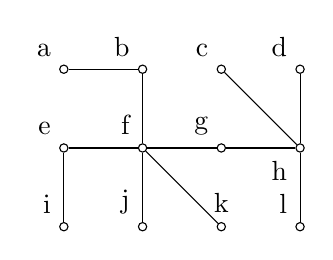
\begin{tikzpicture}
    \begin{scope}
            [vertex/.style={draw,circle,inner sep = 0em, minimum size = 0.3em},
             edgelabel/.style = {fill = white, inner sep = 0.1em, font=\small}]
            \node[vertex, label = above left : a] (a) at (0,0) {};
            \node[vertex, label = above left : b] (b) at (1,0) {};
            \node[vertex, label = above left : c] (c) at (2,0) {};
            \node[vertex, label = above left : d] (d) at (3,0) {};
            \node[vertex, label = above left : e] (e) at (0,-1) {};
            \node[vertex, label = above left : f] (f) at (1,-1) {};
            \node[vertex, label = above left : g] (g) at (2,-1) {};
            \node[vertex, label = below left : h] (h) at (3,-1) {};
            \node[vertex, label = above left : i] (i) at (0,-2) {};
            \node[vertex, label = above left : j] (j) at (1,-2) {};
            \node[vertex, label = above : k] (k) at (2,-2) {};
            \node[vertex, label = above left : l] (l) at (3,-2) {};
            
            \draw[-] (a) to (b);
            \draw[-] (b) to (f);
            \draw[-] (c) to (h);
            \draw[-] (d) to (h);
            \draw[-] (e) to (f);
            \draw[-] (e) to (i);
            \draw[-] (f) to (g);
            \draw[-] (f) to (j);
            \draw[-] (f) to (k);
            \draw[-] (g) to (h);
            \draw[-] (h) to (l);
    \end{scope}
    \end{tikzpicture}
    \end{document}